\section{Introduction to digital signals}

\subsection*{Resources}

The following pages are based on slides developed by Prof. Maraso Yamashiro for the 2015 class on Fourier Analysis. Please work through the slides on the following pages and view the video afterwards.

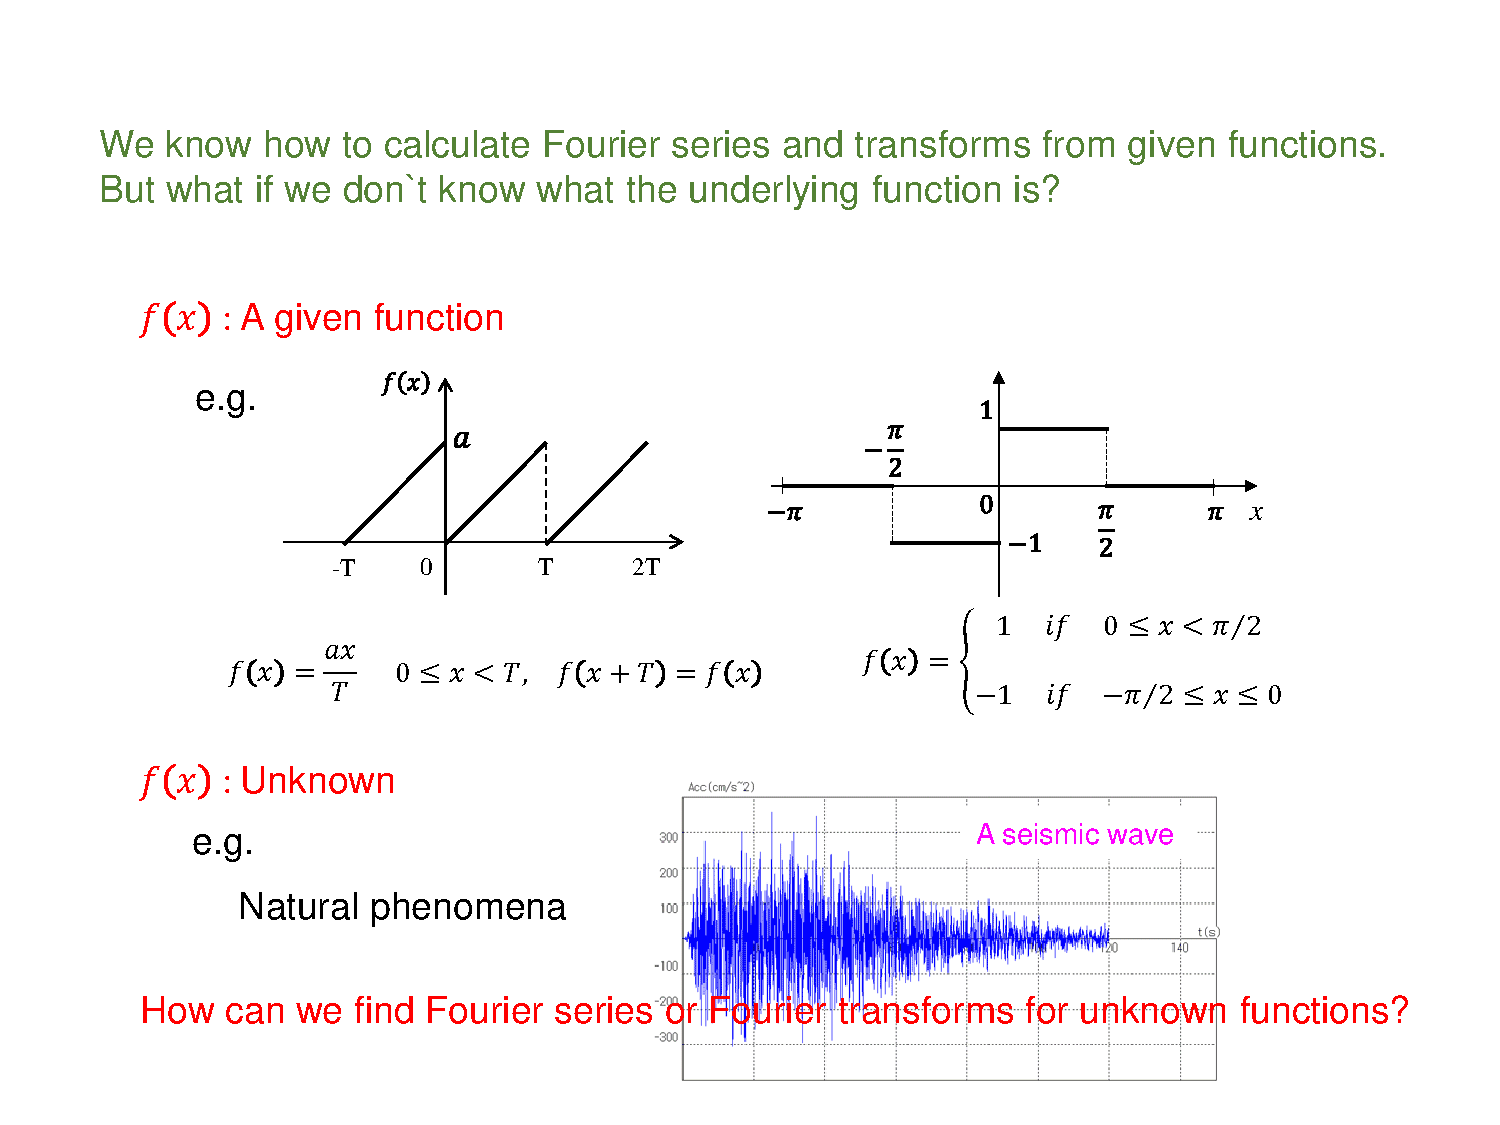
\includepdf[pages=-,pagecommand={},width=\textwidth,nup=1x2,frame=true]{discrete_1-5.pdf}

\begin{itemize}
    \item Video: \url{https://www.youtube.com/watch?v=yWqrx08UeUs&feature=youtu.be&t=47s}
\end{itemize}

\subsection*{Challenge}
1. An audio CD can record frequencies up to 44.1 kHz. Consider how often you would need to sample a sound in order to reproduce frequencies up to 44.1 kHz. What is the highest sampling frequency that experiences aliasing?

2. Write a sentence or two summarising what aliasing is and the Nyquist sampling theorem.

\subsection*{Solutions}
1.\\
\soltwodp{x}{e20c17}

2. Check your answer with your partner and discuss any differences. Ask the teacher if you are unsure.

% Add something on quantisation?




%%%%%%%%%%%%%%%%%%%%%%%%%%%%%%%%%
\newpage
%%%%%%%%%%%%%%%%%%%%%%%%%%%%%%%%%
\section{Discrete Fourier Transform: Coefficients}

\subsection*{Resources}

The following pages are based on slides developed by Prof. Maraso Yamashiro for the 2015 class on Fourier Analysis. The slides have been lightly modified for notation differences.
 %Please follow the derivation on the following pages.
Note that the equation for the discrete Fourier Transform on the top slide of page 90 should read $\hat{f}_n = N c_n = \sum_{k=0}^{N-1} f_k e^{-2 \pi n x_k}$ (not $e^{-inx_k}$) (mistake by the current author, not Prof. Yamashiro).

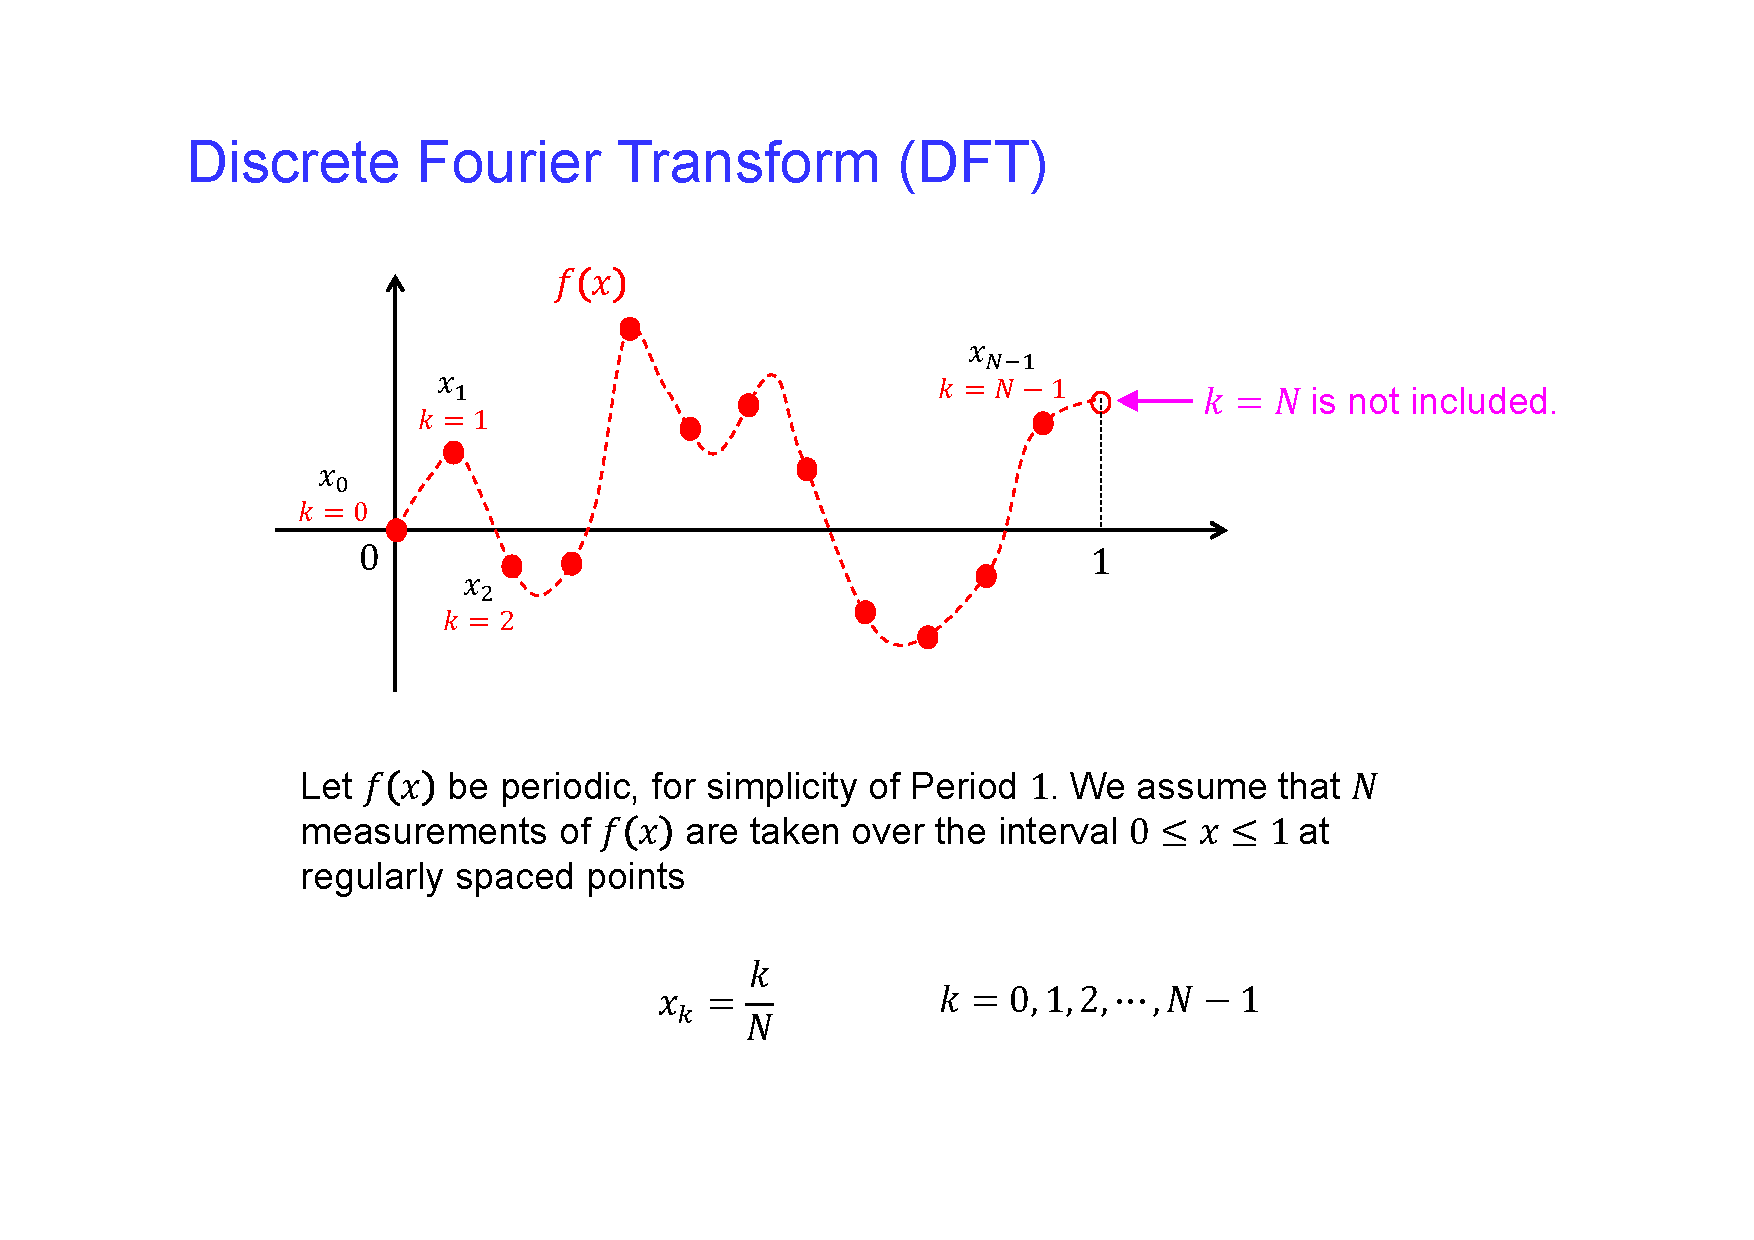
\includepdf[pages=-,pagecommand={},width=\textwidth,nup=1x2,frame=true]{discrete_10-15.pdf}

The challenge below considers sampling of a 1 Hz sine-wave 8 times per second, sampling at time 0, $\frac{1}{8}$, \ldots, $\frac{7}{8}$:

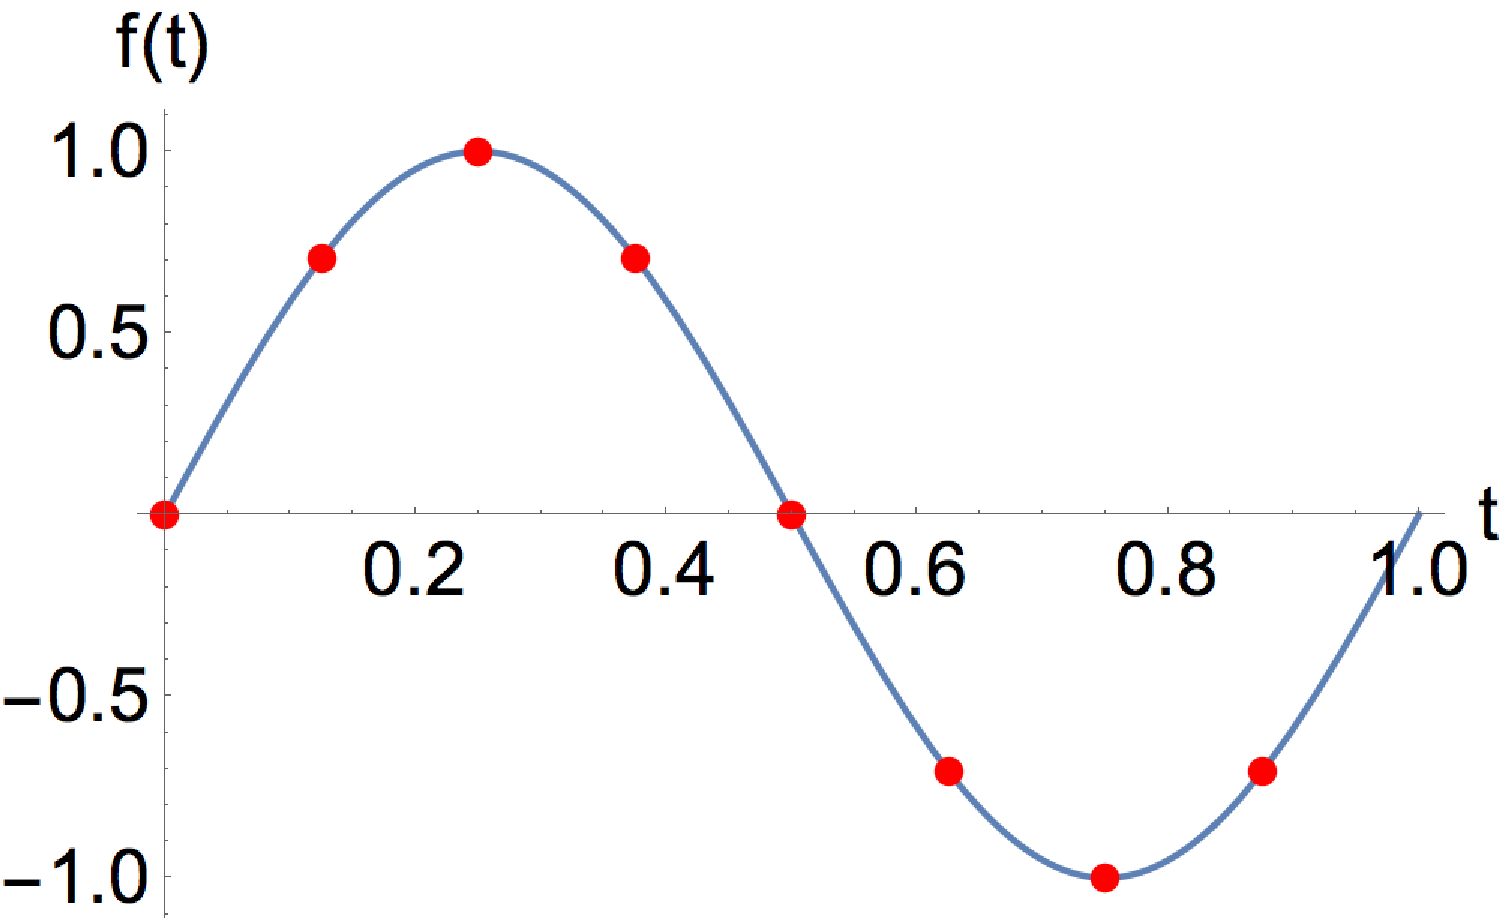
\includegraphics[scale=0.75]{sinedft.png}

This yields sample values of

\begin{equation}
f = \left(
\begin{array}{c}
 0 \\
 1/\sqrt{2} \\
 1 \\
 1/\sqrt{2} \\
 0 \\
 -1/\sqrt{2} \\
 -1 \\
 -1/\sqrt{2} \\
\end{array}
\right)
\end{equation}

\subsection*{Challenge}
Calculate the missing values A-H in the following calculation of the frequency spectrum. To a certain extent you may be able to pattern-match to guess the values, but please be sure that you practise the calculation method too, since that is the main learning objective here.
% NT: Some people do pattern-matching. Maybe need to do a smaller problem where calculation is the only way (can be partial like the previous sensei's 4x4 non-sinusoidal function)


\begin{equation}
    F_8 = 
    \left(
        \begin{array}{cccccccc}
             1 & \textbf{A} & \textbf{B} & 1 & 1 & 1 & 1 & 1 \\
             1 & \textbf{C} & \textbf{D} & -\frac{1+i}{\sqrt{2}} & -1 & -\frac{1-i}{\sqrt{2}} & i & \frac{1+i}{\sqrt{2}} \\
             1 & \textbf{E} & \textbf{F} & i & 1 & -i & -1 & i \\
             1 & -\frac{1+i}{\sqrt{2}} & i & -\frac{1-i}{\sqrt{2}} & -1 & \frac{1+i}{\sqrt{2}} & -i & -\frac{1-i}{\sqrt{2}} \\
             1 & -1 & 1 & -1 & 1 & -1 & 1 & -1 \\
             1 & -\frac{1-i}{\sqrt{2}} & -i & \frac{1+i}{\sqrt{2}} & -1 & -\frac{1-i}{\sqrt{2}} & i & -\frac{1+i}{\sqrt{2}} \\
             1 & i & -1 & -i & 1 & i & -1 & -i \\
             1 & \frac{1+i}{\sqrt{2}} & i & -\frac{1-i}{\sqrt{2}} & -1 & -\frac{1+i}{\sqrt{2}} & -i & -\frac{1-i}{\sqrt{2}} \\
        \end{array}
    \right) 
\end{equation}


\begin{equation}
    \hat{f} =
    \left(
        \begin{array}{c}
             \textbf{G} \\
             \textbf{H} \\
             0 \\
             0 \\
             0 \\
             0 \\
             0 \\
             4 i \\
        \end{array}
    \right)
\end{equation}

\subsection*{Solutions}

Enter imaginary numbers as indicated below. For example: $-1/\sqrt{2}-i/\sqrt{2}$ with a prefix of ``a'' would be entered as ``are(-0.71)im(-0.71)'', $-i$ would be entered as ``are(0.00)im(-1.00)'' and $-1$ would be ``are(-1.00)im(0.00)''.

\textbf{A}\\
\solimagtwodp{a}{95c9e4}

\textbf{B}\\
\solimagtwodp{b}{ec0ffd}

\textbf{C}\\
\solimagtwodp{c}{13085b}

\textbf{D}\\
\solimagtwodp{d}{d01771}

\textbf{E}\\
\solimagtwodp{e}{332be1}

\textbf{F}\\
\solimagtwodp{f}{27b237}

\textbf{G}\\
\solimagtwodp{g}{cbd79b}

\textbf{H}\\
\solimagtwodp{h}{293fff}




%%%%%%%%%%%%%%%%%%%%%%%%%%%%%%%%%
\newpage
%%%%%%%%%%%%%%%%%%%%%%%%%%%%%%%%%
\section{Discrete Fourier Transform: Analysis}

\subsection*{Resources}
Having identified the frequency spectrum, it is possible then to analyse the frequencies of the signal. The video listed below provides a nice introduction into understanding our frequency spectrum. Note that it uses the ``j'' representation of imaginary numbers (instead of ``i'').

\begin{itemize}
    \item Video: \url{https://www.youtube.com/watch?v=mkGsMWi_j4Q}
\end{itemize}

\subsection*{Comment}
The video discusses the phase of the signal as the angle formed by rotating anti-clockwise from an arrow pointing in the positive direction along the real axis. You saw in challenge \ref{sec:ftofsinandcos} how the continuous Fourier transform of a cosine function yields real values and the Fourier transform of a sine function yields imaginary values. Here you can see how phase-shift of a cosine signal leads to real and imaginary solutions and how this can be represented in a real-complex plane.

\subsection*{Challenge}
What is the frequency, magnitude and phase of the sine-wave as determined through our discrete Fourier transform analysis?

\subsection*{Solutions}
\textbf{Frequency}\\
\soltwodp{z}{a78955}

\textbf{Magnitude}\\
\soltwodp{a}{a1e88c}

\textbf{Phase}
\soltwodp{b}{fd9a84}




%%%%%%%%%%%%%%%%%%%%%%%%%%%%%%%%%
\newpage
%%%%%%%%%%%%%%%%%%%%%%%%%%%%%%%%%
\section{Analysing a more complex function: part I}

\subsection*{Challenge}
Considering the signal:
\begin{equation}
    f(t) = \cos(2 \pi t) + \sin(4 \pi t)
\end{equation}

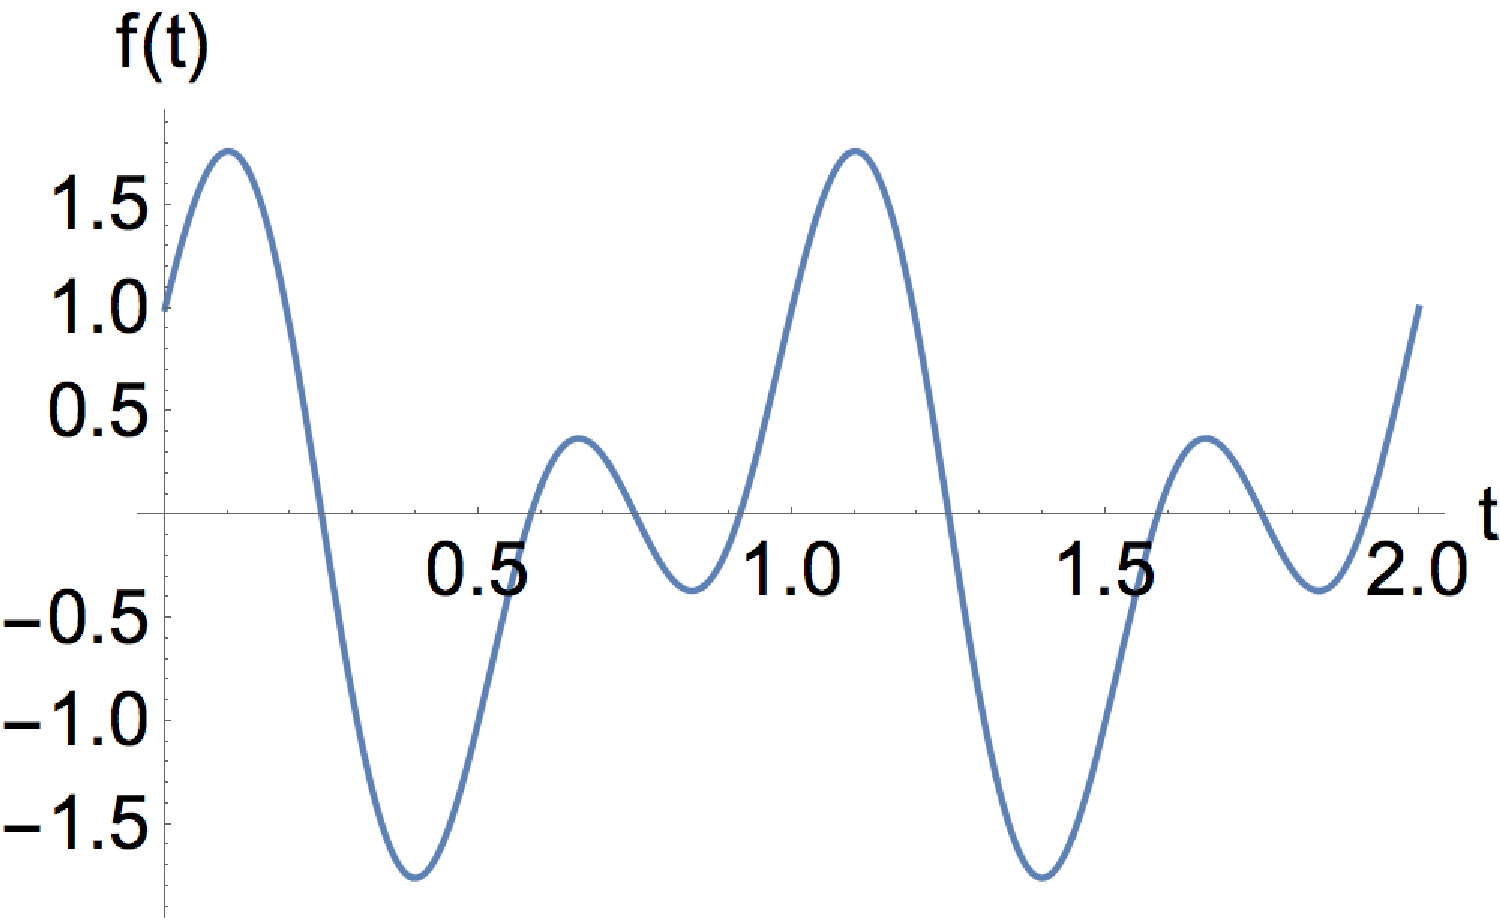
\includegraphics[scale=0.75]{dftcossin.png}

1. What are the two frequencies that make up the signal?

2. What is the fundamental frequency of this signal?

3. What is the maximum sampling frequency at which aliasing will occur for this signal?

\subsection*{Solutions}
\textbf{1. Lower of the two frequencies in Hz}\\
\soltwodp{c}{166765}

\textbf{1. Higher of the two frequencies in Hz}\\
\soltwodp{d}{c22bee}

\textbf{2.}\\
(units: Hz)\\
\soltwodp{f}{6786da}

\textbf{3.}\\
(units: Hz)\\
\soltwodp{e}{0a9397}




%%%%%%%%%%%%%%%%%%%%%%%%%%%%%%%%%
\newpage
%%%%%%%%%%%%%%%%%%%%%%%%%%%%%%%%%
\section{Analysing a more complex function: part II}

\subsection*{Challenge}
Sampling the signal in the previous challenge 8 times per second:

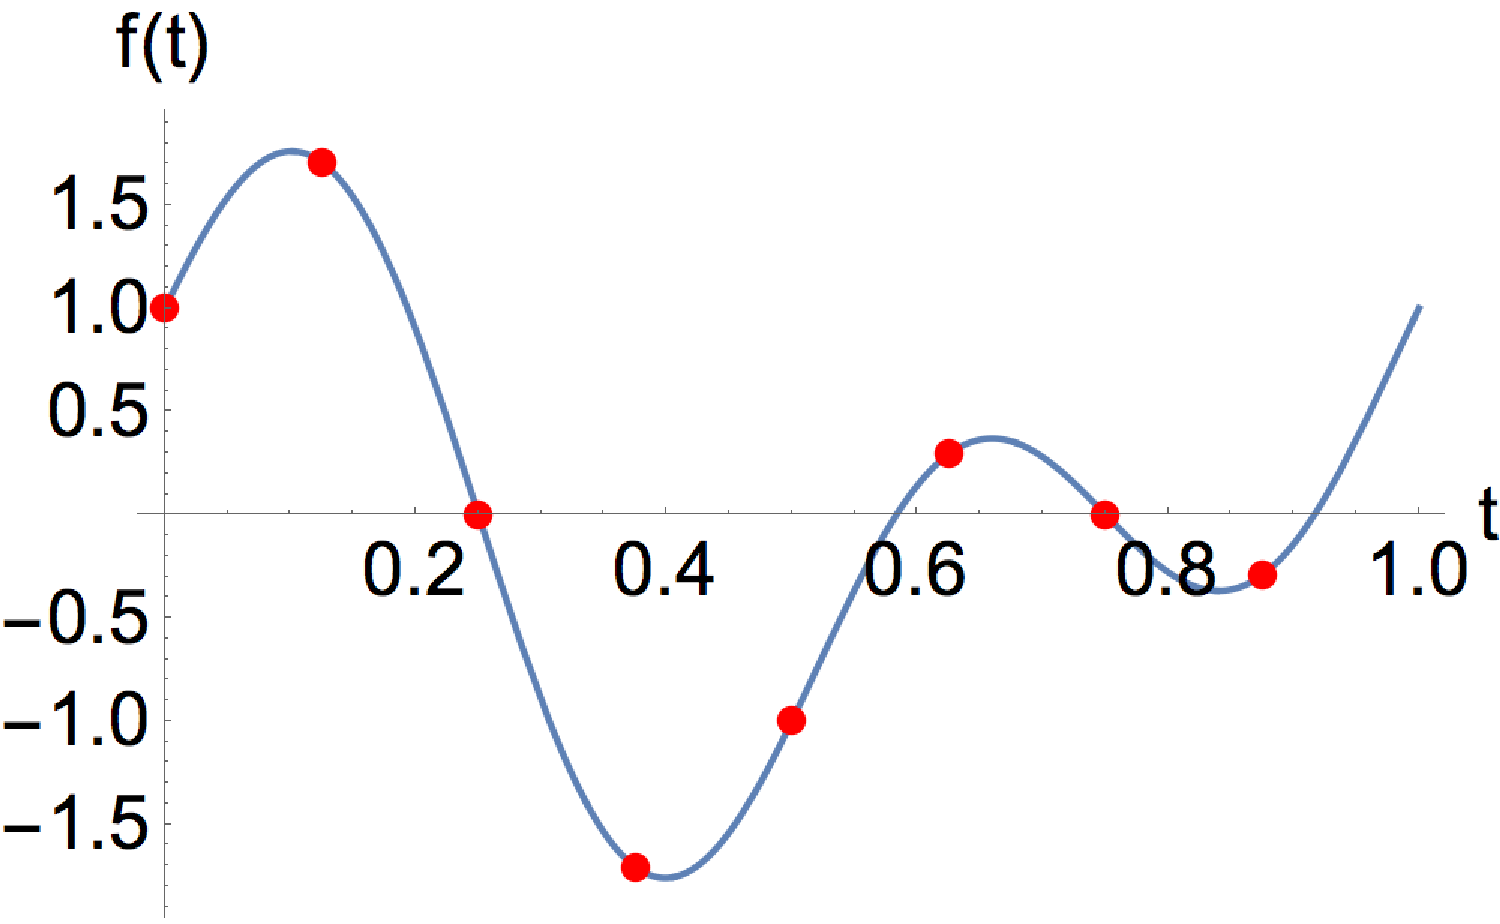
\includegraphics[scale=0.75]{dftcossinsamples.png}

yields values of
\begin{equation}
   \left(
\begin{array}{c}
 1. \\
 1.71 \\
 0. \\
 -1.71 \\
 -1. \\
 0.29 \\
 0. \\
 -0.29 \\
\end{array}
\right) 
\end{equation}

Calculating the matrix F yields

\begin{equation}
   \left(
\begin{array}{cccccccc}
 1 & 1              & 1 & 1 & 1 & 1 & 1 & 1 \\
 1 & (1-i)/\sqrt{2} & \bm{A} & -(1+i)/\sqrt{2} & -1 & (-1+i)/\sqrt{2} & i & (1+i)/\sqrt{2} \\
 1 & \bm{B}         & -1 & i & 1 & -i & -1 & i \\
 1 & -(1+i)/\sqrt{2}& i & (1-i)/\sqrt{2} & -1 & (1+i)/\sqrt{2} & -i & (-1+i)/\sqrt{2} \\
 1 & -1             & 1 & -1 & 1 & -1 & 1 & -1 \\
 1 & (-1+i)/\sqrt{2}& -i & (1+i)/\sqrt{2} & -1 & (1-i)/\sqrt{2} & i & -(1+i)/\sqrt{2} \\
 1 & i              & -1 & -i & 1 & i & -1 & -i \\
 1 & (1+i)/\sqrt{2} & i & (-1+i)/\sqrt{2} & -1 & -(1+i)/\sqrt{2} & -i & (1-i)/\sqrt{2} \\
\end{array}
\right) 
\end{equation}

1. Determine the missing values \textbf{A} and \textbf{B} by calculation.

2. Determine, by calculation, the frequencies with their magnitudes and phases of this signal. In this case, you can know the constituent frequencies, their magnitudes and phases because you know how the signal is made up of two signals. Check that your calculation aligns with your intuition.

\subsection*{Solutions}
\textbf{1. A}\\
\solimagtwodp{a}{223b8b}

\textbf{1. B}\\
\solimagtwodp{b}{df600a}

\textbf{2.} If you are not sure what your intuition should be, or if your answer does not match your intuition, please discuss with your partner or the teacher in class.


% NT: Go the other way to reconstruct a signal. Should spend an entire class on this.
\iffalse
%%%%%%%%%%%%%%%%%%%%%%%%%%%%%%%%%
\newpage
%%%%%%%%%%%%%%%%%%%%%%%%%%%%%%%%%
\section{The limits of DFT calculation}
\label{sec:dftlimits}

\subsection*{Resources}
Practically, the DFT is calculated using the Fast Fourier Transform (FFT). The reason is that the number of operations grows with the square of the number of samples which is unsustainable for typical signals.

The following pages are based on slides developed by Prof. Maraso Yamashiro for the 2015 class on Fourier Analysis, and highlight this problem quantitatively.

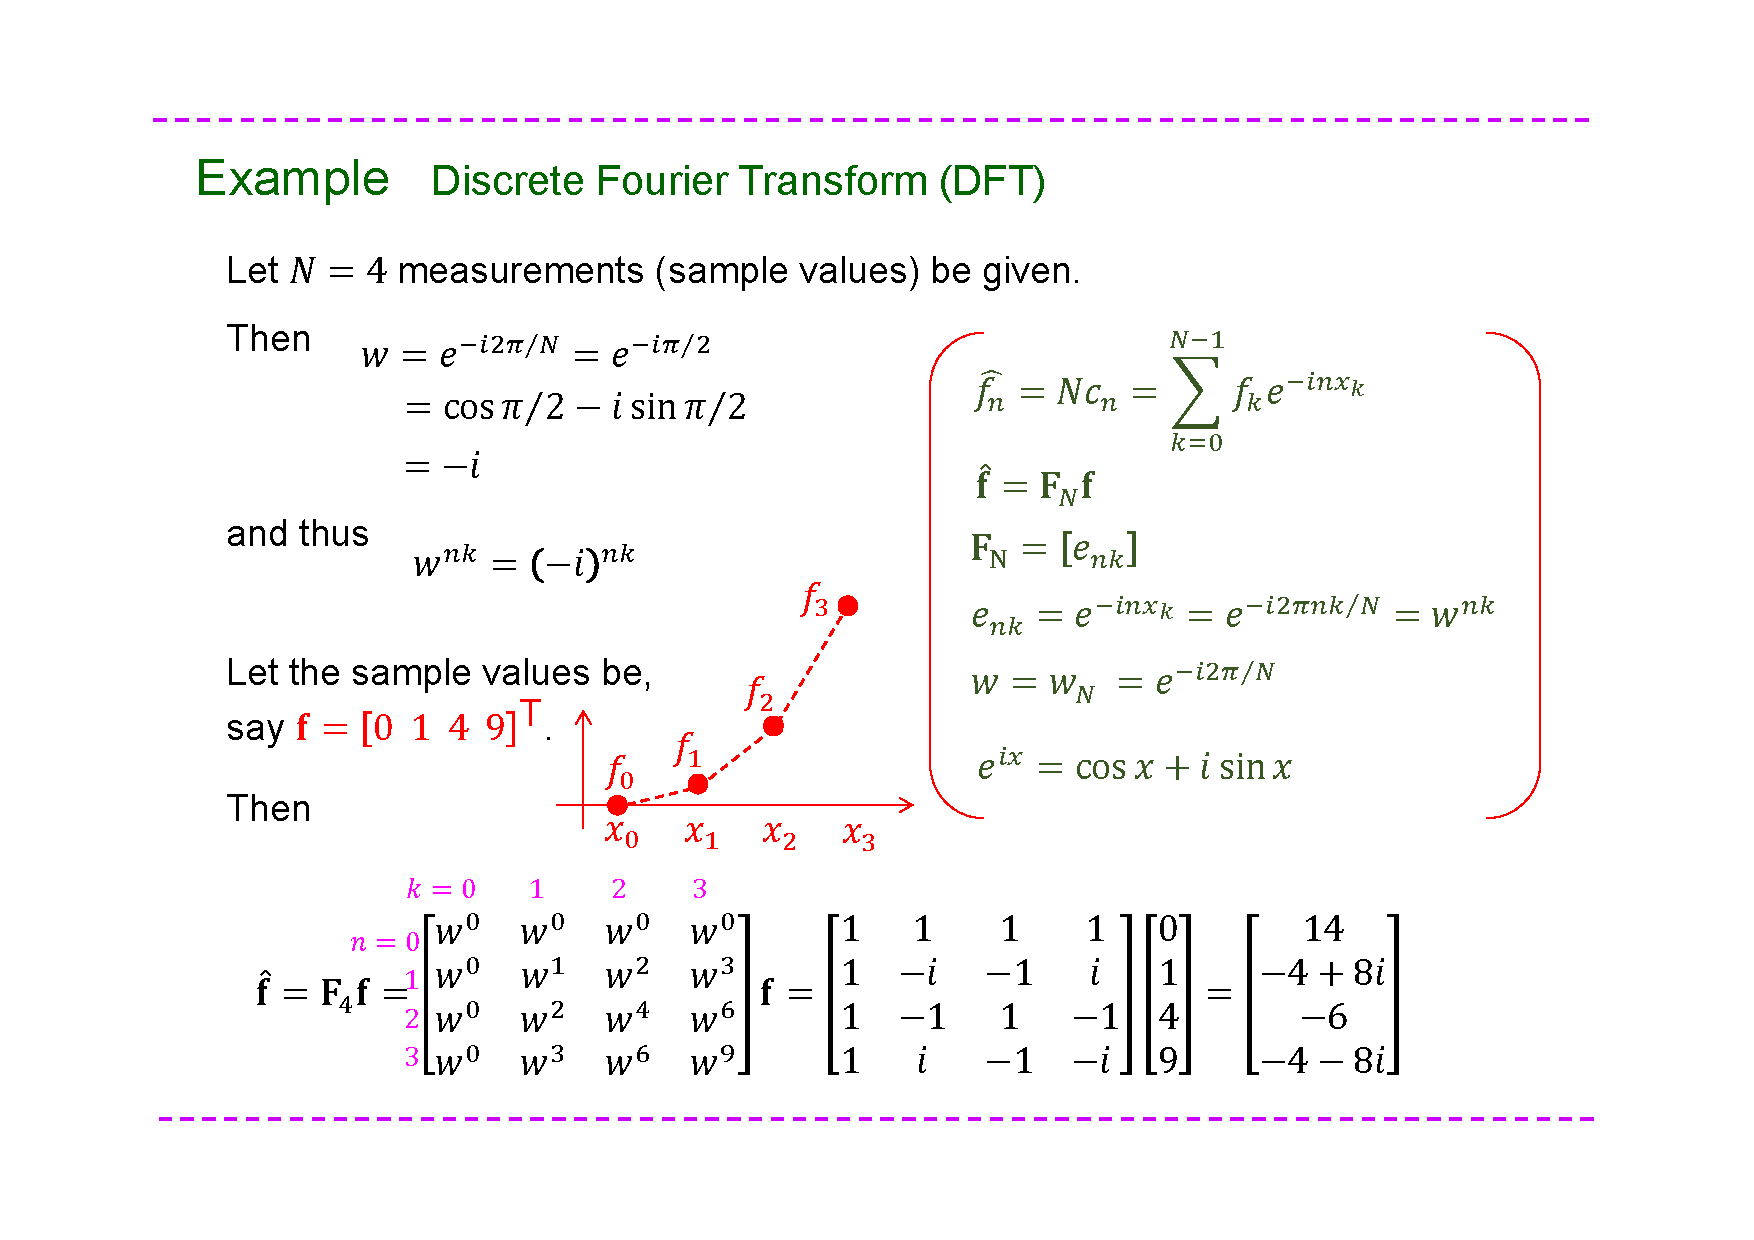
\includepdf[pages=-,pagecommand={},width=\textwidth,nup=1x2,frame=true]{fft_1-4.pdf}

\subsection*{Challenge}
Considering a signal sampled at 22 kHz, how many multiplications are required to calculate $F$ in the calculation $\bm{\hat{f}} = F \bm{f}$?

\subsection*{Solutions}
\solscitwodp{c}{eb9210}




%%%%%%%%%%%%%%%%%%%%%%%%%%%%%%%%%
\newpage
%%%%%%%%%%%%%%%%%%%%%%%%%%%%%%%%%
\section{The concepts of the FFT}

\subsection*{Resources}
The Cooley and Tukey algorithm for calculating the FFT is not that complicated, but can get very messy and it takes some time to really understand it. Therefore, we will limit ourselves to understanding some basic concepts upon which it is built.

The main concept is that many of the elements in the Fourier matrix are repetitive. For example, you can notice the symmetry about the diagonal in the $F_4$ matrix:

\begin{equation}
   F_4 = \left(
\begin{array}{cccc}
    1 & \tcr{1} & \tcr{1} & \tcr{1} \\
    \tcb{1} & -i & \tcr{-1} & \tcr{i} \\
    \tcb{1} & \tcb{-1} & 1 & \tcr{-1} \\
    \tcb{1} & \tcb{i} & \tcb{-1} & -i \\
\end{array}
\right) 
\end{equation}

One key concept therefore is that once we have calculated an element of the matrix, we don't need to calculate it again for elements that will turn out to be the same. The key question then becomes: how do we determine which elements will be repetitions of which other elements?

The ``twiddle factor'' shows how elements of matrix $F_N$ (ie, $w^{nk}$) are repeated. This can be visualised as points on a circle on the real-imaginary plane as the following slides from Prof. Maraso Yamashiro show.

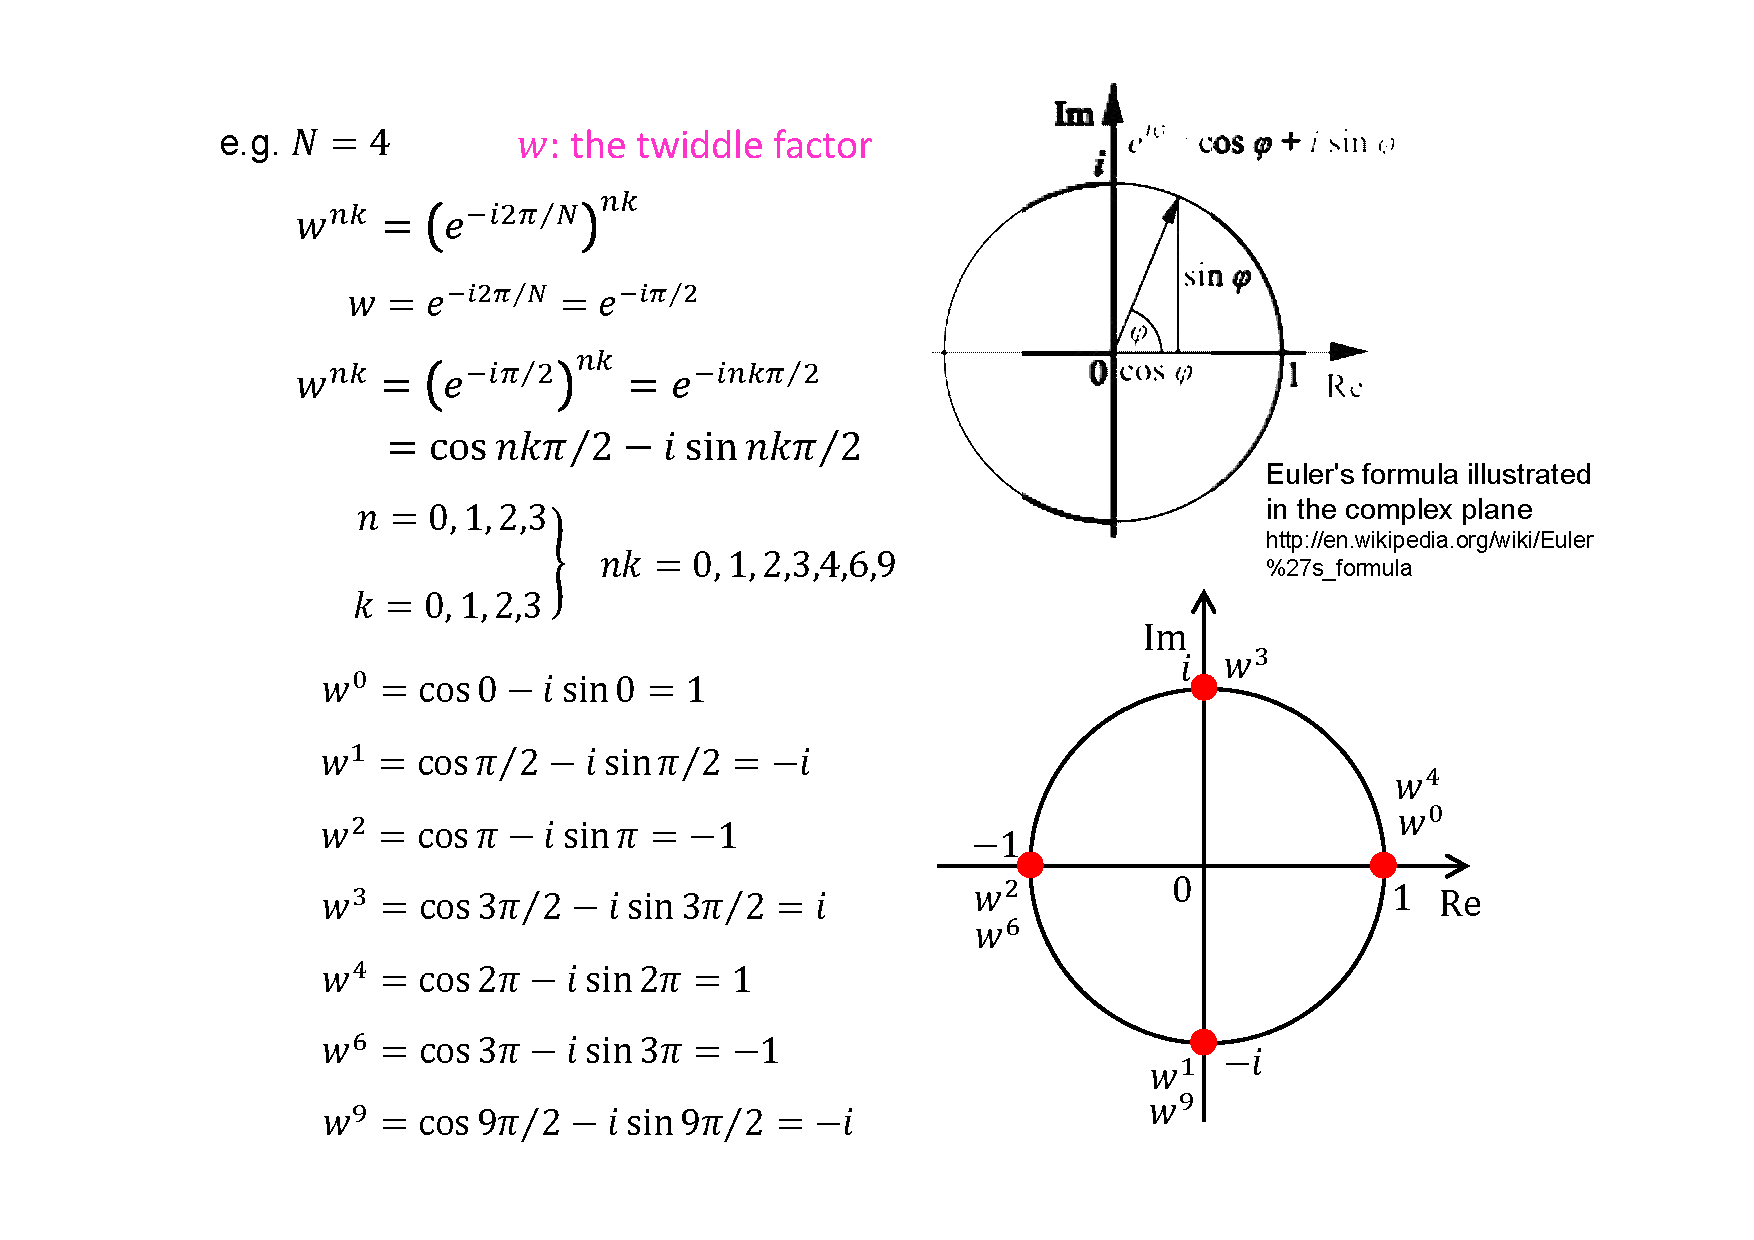
\includepdf[pages=-,pagecommand={},width=\textwidth,nup=1x2,frame=true]{fft_6-7.pdf}

First one can notice that repeated terms are consistently even or odd. For example, for $N=8$ it was seen that $w^0$, $w^8$, $w^{16}$ and $w^{24}$ all share the same value ($=1$) while $w_7$ and $w_{15}$ share the same (off-axis) value. You will notice however that simply breaking the functions into odd and even terms is not enough to unambiguously define the values of the twiddle factors, since even and odd terms can each still have multiple values.

One can take advantage of this symmetry (in ways not explained here) by taking the even-numbered terms and odd-numbered terms of the signal-vector $\bm{f}$ to create two new vectors, each of half the length of the original signal-vector:

\begin{align}
    \bm{f_{even}} &= [f_0, f_2, \dots, f_{N-2}]^T \\
    \bm{f_{odd}} &= [f_1, f_3, \dots, f_{N-1}]^T
\end{align}

Then renumbering the terms back to $0, 1, 2, \dots, N/2-1$:

\begin{align}
    \bm{f_{even}} &= [f_{ev,0}, f_{ev,1}, \dots, f_{ev,N/2-1}]^T \\
    \bm{f_{odd}} &= [f_{od,0}, f_{od,1}, \dots, f_{od,N/2-1}]^T \\
\end{align}

This can then be repeated, taking the even- and odd-numbered terms of $\bm{f_{even}}$ to make two more vectors of half-length, and doing the same for $\bm{f_{odd}}$ so we now have 4 vectors each $1/4$ the length of the original signal-vector $\bm{f}$. This is repeated until there are $N/2$ vectors each of length $2$.

Although beyond the scope of the explanation here, this ultimately allows one to take advantage of the repetitive nature of the twiddle factor, reducing the scaling of the number of multiplications drastically from $N^2$ to $Nlog_2 N$, as shown in the following slide from Prof. Maraso Yamashiro:

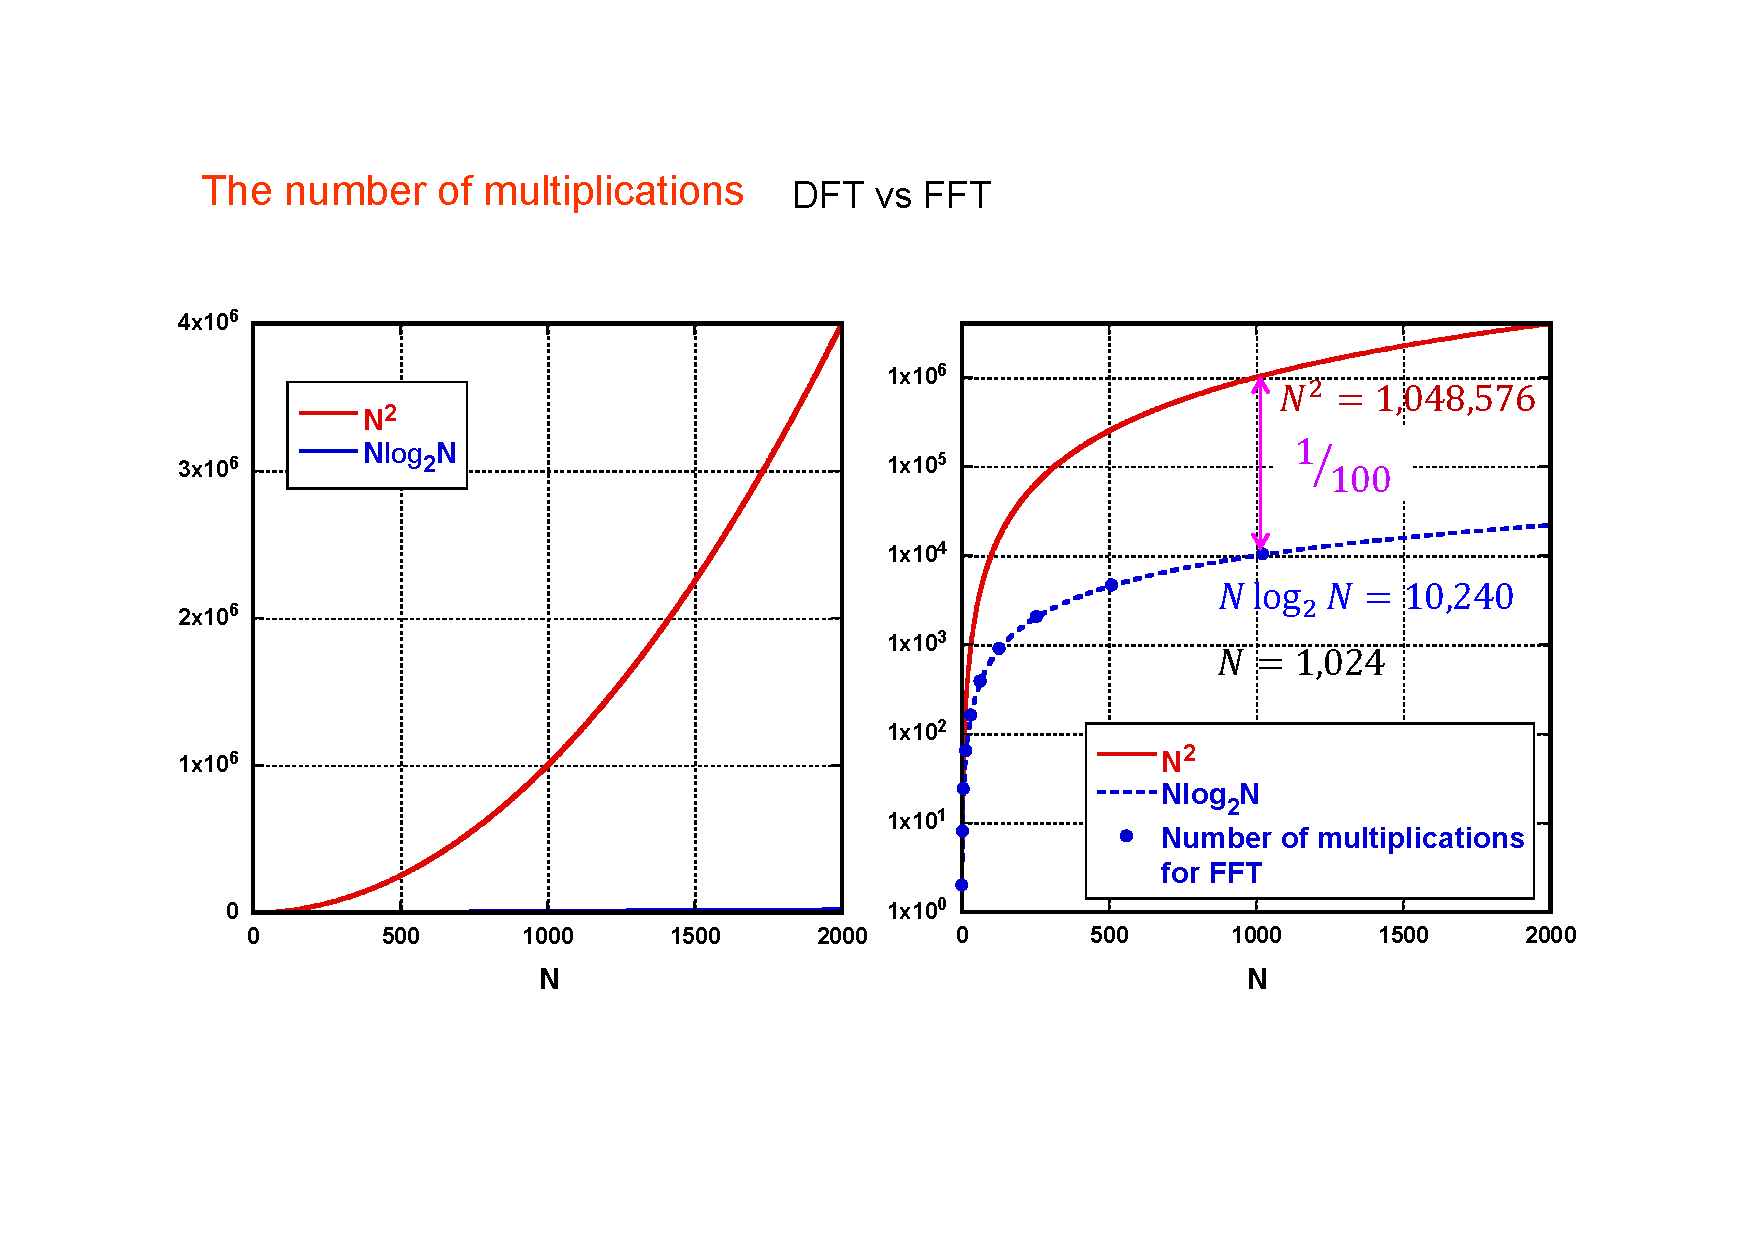
\includepdf[pages=-,pagecommand={},width=\textwidth,nup=1x2,frame=true]{fft_28.pdf}

A further point to note is that, in order to continuously divide the signal in half until each vector is length $2$, the original signal must be of length $2^p$ where p is some integer. For example, a signal of length $8$ such as $\bm{[1,2,3,4,5,6,7,8]}$ can be halved once into two vectors of length four ($\bm{[1,3,5,7]}$ and $\bm{[2,4,6,8]}$) and then again into four vectors of length two ($\bm{[1,5]}$, $\bm{[3,7]}$, $\bm{[2,6]}$, $\bm{[4,8]}$). If the vector is of length 9 however, such as $\bm{[1,2,3,4,5,6,7,8,9]}$, the signal cannot be divided into two signals of \emph{equal length}.

This problem is overcome through the use of \emph{zero-padding}. In the example in the previous paragraph, the signal of length $9$ would simply have seven zeros added to it at the end to create a signal of total length $16$ ($\bm{[1,2,3,4,5,6,7,8,9,0,0,0,0,0,0,0]}$), which could then be halved three times into eight vectors of length $2$.

\subsection*{Challenge}
1. Considering the signal that generated the spectrum in challenge \ref{sec:dftlimits}, how many zeros must be added to the end of the sampled signal to permit FFT to be performed?

2. How many times can the padded signal be halved?

3. How many multiplications does this signal require under FFT?

4. Considering the original unpadded signal, how many times more multiplications are required under standard DFT compared to processing under FFT?

\subsection*{Solutions}
\textbf{1}\\
\solscitwodp{d}{293b72}

\textbf{2}\\
\soltwodp{e}{f5df85}

\textbf{3}\\
491,520

\textbf{4}\\
984.70
\fi
